\documentclass{beamer}

\mode<presentation> {

% The Beamer class comes with a number of default slide themes
% which change the colors and layouts of slides. Below this is a list
% of all the themes, uncomment each in turn to see what they look like.

%\usetheme{default}
%\usetheme{AnnArbor}
%\usetheme{Antibes}
%\usetheme{Bergen}
%\usetheme{Berkeley}
%\usetheme{Berlin}
%\usetheme{Boadilla}
%\usetheme{CambridgeUS}
%\usetheme{Copenhagen}
%\usetheme{Darmstadt}
\usetheme{Dresden}
%\usetheme{Frankfurt}
%\usetheme{Goettingen}
%\usetheme{Hannover}
%\usetheme{Ilmenau}
%\usetheme{JuanLesPins}
%\usetheme{Luebeck}
%\usetheme{Madrid}
%\usetheme{Malmoe}
%\usetheme{Marburg}
%\usetheme{Montpellier}
%\usetheme{PaloAlto}
%\usetheme{Pittsburgh}
%\usetheme{Rochester}
%\usetheme{Singapore}
%\usetheme{Szeged}
%\usetheme{Warsaw}

% As well as themes, the Beamer class has a number of color themes
% for any slide theme. Uncomment each of these in turn to see how it
% changes the colors of your current slide theme.

%\usecolortheme{albatross}
%\usecolortheme{beaver}
%\usecolortheme{beetle}
%\usecolortheme{crane}
%\usecolortheme{dolphin}
%\usecolortheme{dove}
%\usecolortheme{fly}
%\usecolortheme{lily}
%\usecolortheme{orchid}
%\usecolortheme{rose}
%\usecolortheme{seagull}
%\usecolortheme{seahorse}
\usecolortheme{whale}
%\usecolortheme{wolverine}

%\setbeamertemplate{footline} % To remove the footer line in all slides uncomment this line
%\setbeamertemplate{footline}[page number] % To replace the footer line in all slides with a simple slide count uncomment this line

%\setbeamertemplate{navigation symbols}{} % To remove the navigation symbols from the bottom of all slides uncomment this line
}

\usepackage{graphicx} % Allows including images
\usepackage{booktabs} % Allows the use of \toprule, \midrule and \bottomrule in tables
\usepackage[backend=bibtex,natbib=true,sorting=none,style=nature]{biblatex}
\bibliography{../MT.bib}

%----------------------------------------------------------------------------------------
%	TITLE PAGE
%----------------------------------------------------------------------------------------

\title[Ultrafast manipulation of antiferromagnetic insulators]{Ultrafast manipulation of Heisenberg exchange and Dzyaloshinskii Moriya interactions in antiferromagnetic insulators} % The short title appears at the bottom of every slide, the full title is only on the title page

%\author{Juan Manuel Losada Sosnovsky} % Your name
%\autoref{asdf}{asdf}
%\author[author1]{author1\inst{1}\\[1ex]  {\small supervisor1\inst{1,2}}}
\author[Juan Manuel Losada Sosnovsky]{Juan Manuel Losada Sosnovsky\\[5mm]{\small Supervisors: Arne Brataas and Alireza Qaiumzadeh}}
\institute[NTNU] % Your institution as it will appear on the bottom of every slide, may be shorthand to save space
{
QuSpin (NTNU)
}
\date{\today} % Date, can be changed to a custom date
\newcommand{\bs}[1] {\boldsymbol{#1}}
\begin{document}

\begin{frame}
\titlepage % Print the title page as the first slide
\end{frame}

%----------------------------------------------------------------------------------------
%	PRESENTATION SLIDES
%----------------------------------------------------------------------------------------

%------------------------------------------------
\section{First Section} % Sections can be created in order to organize your presentation into discrete blocks, all sections and subsections are automatically printed in the table of contents as an overview of the talk
%------------------------------------------------

\subsection{Subsection Example} % A subsection can be created just before a set of slides with a common theme to further break down your presentation into chunks

\begin{frame}
\frametitle{Spintronics}
Study and use the intrinsic spin of the electrons, in addition to their charge, to build devices. Example: Magnetoresistive random access memory.

%\begin{figure}
%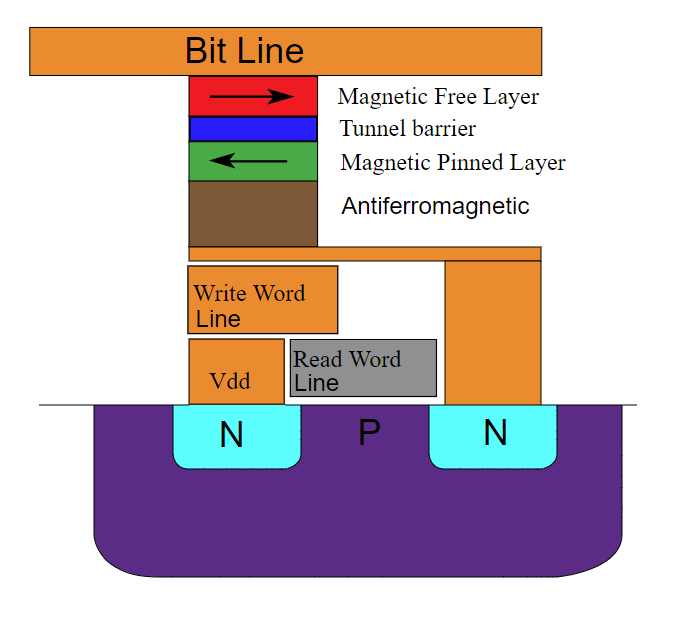
\includegraphics[width=0.5\linewidth]{../Figures/fm_device.png}
%\caption{Source: Wikipedia}
%\end{figure}

\begin{figure}
  \begin{minipage}[c]{0.6\textwidth}
    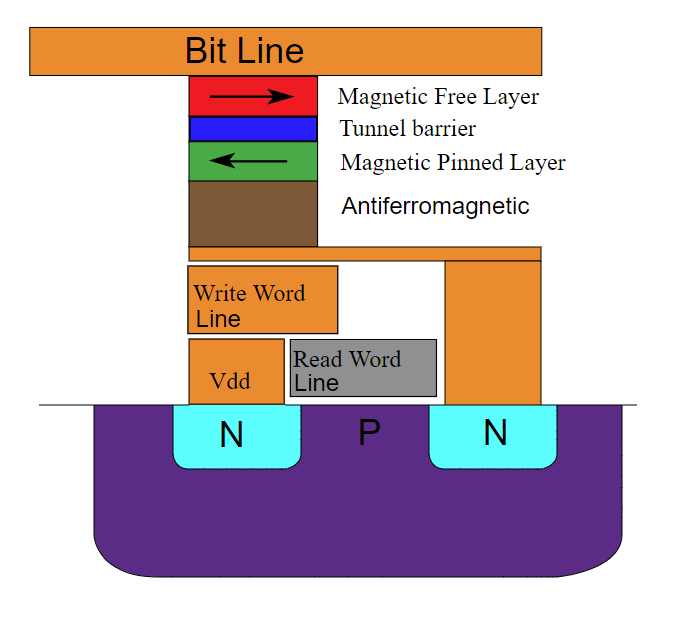
\includegraphics[width=\textwidth]{../Figures/fm_device.png}
  \end{minipage}\hfill
  \begin{minipage}[c]{0.2\textwidth}
    \caption{Source: Wikipedia} \label{fig:1}
  \end{minipage}
\end{figure}

\end{frame}

%------------------------------------------------

\begin{frame}
\frametitle{Antiferromagnetic Spintronics}
The development of information technology demands devices with high storage density, high energy efficiency and high write-read speeds. Antiferromagnets have appear as a natural alternative to ferromagnets due to some advantages: 
\begin{itemize}
\item Robustness against magnetic disturbances.
\item No hysteresis loss.
\item Produce no stray fields.
\item Ultrafast dynamics (femtosecond).
\end{itemize}
\end{frame}

\begin{frame}
\frametitle{Antiferromagnetic Spintronics}

\begin{figure}
  \begin{minipage}[c]{0.6\textwidth}
    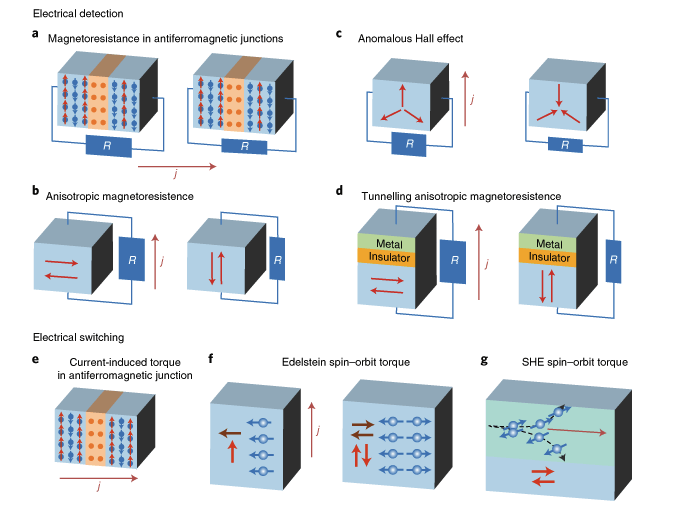
\includegraphics[width=\textwidth]{../Figures/afm_device.png}
  \end{minipage}\hfill
  \begin{minipage}[c]{0.2\textwidth}
    \caption{Source: Nature, Spin transport and spin torque in antiferromagnetic devices} \label{fig:2}
  \end{minipage}
\end{figure}

\end{frame}

%------------------------------------------------

\begin{frame}
\frametitle{Spin models}
\begin{block}{Heisenberg model}
\begin{equation} 
\hat{H} = \sum_{\langle i,j \rangle} J \bs{S}_i \bs{S}_j \nonumber
\end{equation}
In antiferromagnets $J > 0$ ($J < 0$ for ferromagnets). Mentink, J. H. et al. showed that it is possible to manipulate the exchange constant by applying a laser field. $J = J_0 + \Delta J$.
\end{block}
\end{frame}

%------------------------------------------------

\begin{frame}
\frametitle{Spin models}
The Dzyaloshinskii-Moriya interaction (DMI):
\begin{equation*}
\bs{D}_{ij}\bs{S}_i\times\bs{S}_j
\end{equation*}
\begin{itemize}
\item Arises from the spin orbit coupling.
\item It favours canted order, i.e. weak ferromagnetism in AFM.
\item Enables topological objects such as chiral skyrmions and chiral domain walls.
\end{itemize}
\end{frame}

%------------------------------------------------

\begin{frame}
\frametitle{Spin models}
\begin{block}{Heisenberg model with DMI}
\begin{equation} 
\hat{H} = \sum_{\langle i,j \rangle} J \bs{S}_i \bs{S}_j + \sum_{\langle i,j \rangle} \vec{D}_{ij}\bs{S}_i \times \bs{S}_j\nonumber
\end{equation}

The ratio between the exchange interaction and the DMI controls the tilt angle of the canted spins.

\begin{figure}
  \begin{minipage}[c]{0.6\textwidth}
    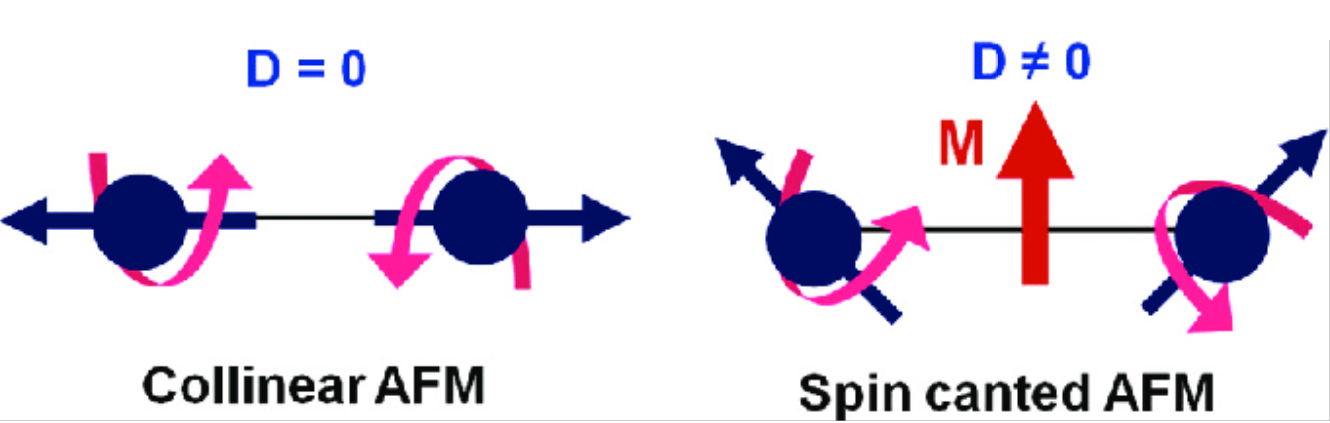
\includegraphics[width=\textwidth]{../Figures/dmi_canting.png}
  \end{minipage}\hfill
  \begin{minipage}[c]{0.2\textwidth}
    \caption{Source: Nanoscale} \label{fig:3}
  \end{minipage}
\end{figure}

\end{block}
\end{frame}

%------------------------------------------------

\begin{frame}
\frametitle{Spin models}
If we can manipulate $J$ and $D$ we can control the canting angle.
\begin{figure}
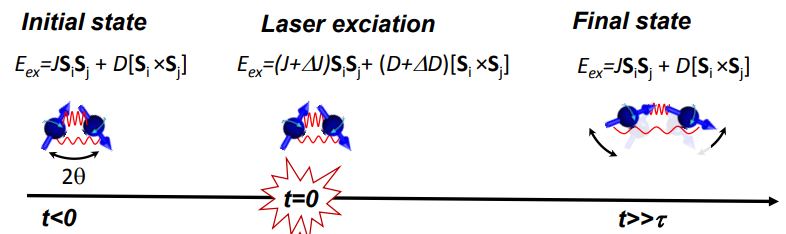
\includegraphics[width=1\linewidth]{../Figures/canted_afm.png}
\caption{Source: Kimmel presentation}
\end{figure}
\end{frame}

%------------------------------------------------

%\begin{frame}
%\frametitle{Manipulation of the spin state}
%We need $\frac{J}{D} \neq \frac{J+\Delta J}{D+\Delta D}$.
%\\[10mm]
%However, $\frac{J}{D} = \frac{J+\Delta J}{D+\Delta D}$.
%\end{frame}

%------------------------------------------------

\begin{frame}
\frametitle{Model}
Strongly correlated electrons in a planar honeycomb lattice can be described by:
\begin{block}{Kane-Mele-Hubbard model}
\begin{equation}
\hat{H} = - t_1\sum_{\langle i,j \rangle, \sigma} \hat{c}_{i \sigma}^\dagger \hat{c}_{j \sigma} -
	\sum_{\langle \langle i,j \rangle \rangle, \sigma, \sigma'}(\delta_{\sigma,\sigma'}t_2 - i\Delta\nu_{ij}\sigma^z_{\sigma, \sigma'})\hat{c}_{i \sigma}^\dagger \hat{c}_{j \sigma'} + \text{U}\hat{D}\nonumber
\end{equation}

Where $\hat{D} = \sum_{i=1}^M \hat{n}_{i\uparrow}\hat{n}_{i\downarrow}$ is the doublon number operator.

\end{block}
\end{frame}

%------------------------------------------------

\begin{frame}
\frametitle{Model}
\begin{figure}[t]
\centering
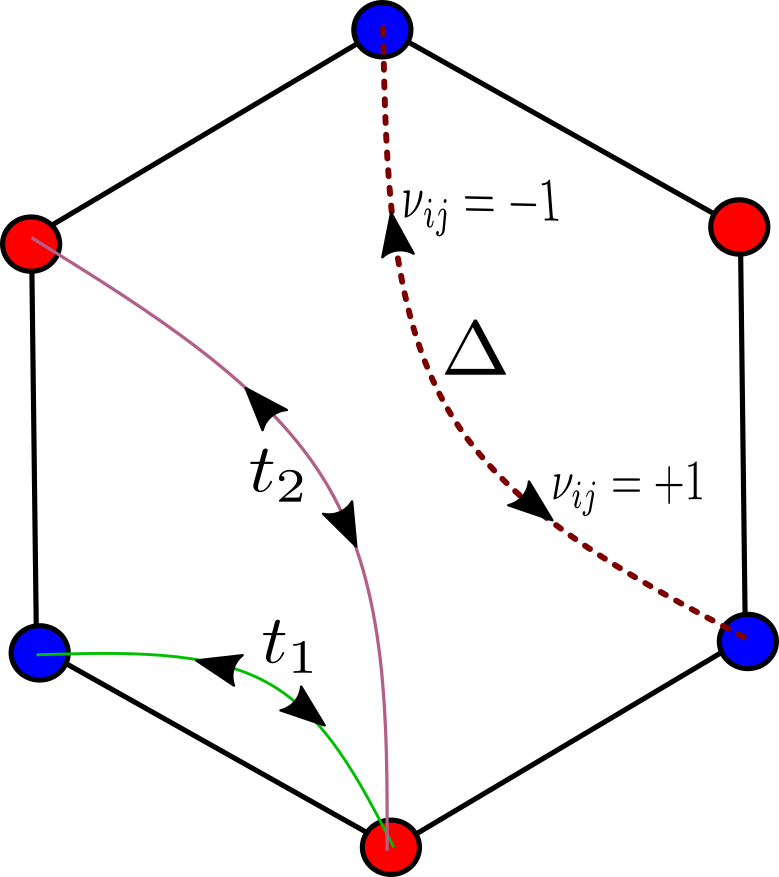
\includegraphics[width=0.45\columnwidth]{../Paper/kmh.png}
\caption{A honeycomb cell with NN hopping $t_1$, NNN hopping $t_2$, intrinsic SOI $\Delta$, and $\nu_{ij} = \pm 1$ for clockwise and counterclockwise hopping.}
\label{fig1}
\vspace*{-6pt}
\end{figure}
\end{frame}

%------------------------------------------------

\begin{frame}
\frametitle{Model}
The effective spin Hamiltonian in the strongly correlated regime takes the form:
\begin{equation}
\hat{H}_{\text{eff}} = \sum_{\langle i,j \rangle} J_{1}\bs{S}_i\bs{S}_j + \sum_{\langle \langle i,j \rangle \rangle} \left\{ J_{2}\bs{S}_i\bs{S}_j + \bs{D}_{2,ij} \bs{S}_i \times \bs{S}_j + \bs{S}_i \bs{\Gamma} \bs{S}_j \right\} \nonumber
\end{equation}
With:
\begin{align*}
&J_{1(2)} = \frac{2t_{1(2)}^2}{U}, \\
&\bs{\Gamma} =\frac{2\Delta^2}{U} \text{diag}(-1,-1,1),\\
&\bs{D}_{ij} = \frac{4 t_2 \Delta}{U}\nu_{ij}  \hat{\mathrm{e}}_z.
\end{align*}

\end{frame}

%------------------------------------------------

\begin{frame}
\frametitle{Method}
\begin{equation*}
\hat{H} = -\hat{T} + \text{U}\hat{D}
\end{equation*}
$\hat{T}$ is a hopping operator, and $\hat{D}$ is the doublon number operator.
\begin{align*}
\hat{D} &= \sum_{i=1}^M \hat{n}_{i\uparrow}\hat{n}_{i\downarrow} \\
\hat{T} &= \sum_{i,j, \sigma, \sigma'} t_{ij}^{\sigma \sigma'} \hat{c}_{i \sigma}^\dagger \hat{c}_{j \sigma'}
\end{align*}
$\text{U} \gg t_{ij}^{\sigma \sigma'}$, strongly correlated regime.
\end{frame}

%------------------------------------------------

\begin{frame}
\frametitle{Method}
To account for the laser illumination we use several techniques:
\begin{itemize}
\item Peierls substitution.
\item Apply time dependent unitary transformation.
\item Expand unitary transformation and transformed Hamiltonian.
\item Determine unitary transformation.
\end{itemize}
\end{frame}

%------------------------------------------------

\begin{frame}
\frametitle{Peierls substitution}
In the presence of a vector potential $\bs{A}(t)$ the hopping amplitudes acquire a time dependent phase:
\begin{equation*}
\label{TimeDepHopping}
t_{ij}^{\sigma \sigma'}(t) = t_{ij}^{\sigma \sigma'} e^{ie\bs{R}_{ij}\bs{A}(t)}
\end{equation*}
The Hamiltonian is time dependent.
\end{frame}

%------------------------------------------------

\begin{frame}
\frametitle{Unitary transformation}
Apply $\hat{U}(t) = e^{-i\hat{S}(t)}$,

\begin{equation*}
\hat{H}'(t) = e^{i\hat{S}(t)} \hat{H}(t) e^{-i\hat{S}(t)} - e^{i\hat{S}(t)} id_t e^{-i\hat{S}(t)}
\end{equation*}
The goal is $\hat{H}'(t)$ to be block diagonal in $\hat{D}$ up to certain order in the hopping amplitudes.
\end{frame}

%------------------------------------------------

\begin{frame}
\frametitle{Expand transformed Hamiltonian}
Formally $\hat{T}(t) = \eta\hat{T}(t)$, where $\eta$ plays the role of a bookkeeping parameter in the perturbative expansion.
\begin{align*}
\hat{S}(t) &= \sum_\nu \eta^\nu \hat{S}^{(\nu)}(t) \\
\hat{H}'(t) &= \sum_\nu \eta^\nu \hat{H}'^{(\nu)}(t)
\end{align*}

The transformed Hamiltonian can be written:

\begin{equation*} 
\hat{H}'(t) = \sum_m \frac{1}{m!} \text{ad}_{i\hat{S}(t)}^m \left( \hat{H}(t) - \sum_n \frac{1}{(n+1)!}\text{ad}_{-i\hat{S}(t)}^n (d_t \hat{S}(t)) \right)
\end{equation*}
\end{frame}

%------------------------------------------------

\begin{frame}
\frametitle{Determine unitary transformation}
We decompose the hopping operator as $\hat{T}(t) = \sum_{d,m} \hat{T}_{d,m}e^{im\omega t}$, where $\hat{T}_{d,m}$ changes the doublon number by $d$.
\begin{align*}
\hat{H}'^{(0)}(t) &= \text{U}\hat{D} \\
\hat{H}'^{(1)}(t) &= -\sum_m \hat{T}_{0,m}(t)e^{im\omega t} \\
\hat{H}'^{(2)}(t) &= \frac{1}{2}\sum_{mn} \left( \frac{\left[\hat{T}_{1n}, \hat{T}_{-1(m-n)} \right]}{\text{U}+n\omega} - \frac{\left[\hat{T}_{-1n}, \hat{T}_{1(m-n)} \right]}{\text{U}-n\omega} \right) e^{im\omega t}
\end{align*}
\end{frame}

%------------------------------------------------

\begin{frame}
\frametitle{Projecting onto the low energy subspace}
In the strongly correlated limit we can assume that the Hamiltonian acts only within the $d=0$ subspace, i.e. $\hat{H}_{\text{eff}}=\langle \hat{P}_0\hat{H}'(t)\hat{P}_0 \rangle$. Obtaining:
\begin{equation*}
\hat{H}_{\text{eff}} = - \sum_{i,j, \sigma_1, \sigma_2, \sigma_3, \sigma_4}\hat{c}_{i \sigma_1}^\dagger \hat{c}_{j \sigma_2} \hat{c}_{j \sigma_3}^\dagger \hat{c}_{i \sigma_4} t_{ij}^{\sigma_1 \sigma_2} t_{ji}^{\sigma_3 \sigma_4} \left\{ \sum_{n} \frac{\mathcal{J}_{n}^2(\alpha_{ij})}{\text{U}+n\omega} \right\}
\end{equation*}
Where $\alpha_{ij} = e\bs{R}_{ij}\bs{A}$.
\end{frame}

%------------------------------------------------

\begin{frame}
\frametitle{Results}
If we apply this procedure to the Kane Mele Hubbard model, we get:
\begin{align*}
\tilde{H}_{\text{S}}(\omega) =& \sum_{\langle i,j \rangle} \tilde{J}_{1,ij} \bs{S}_i\bs{S}_j + \sum_{\langle \langle i,j \rangle \rangle} \left\{ \tilde{J}_{2,ij}\bs{S}_i\bs{S}_j + \bs{S}_i \tilde{\bs{\Gamma}}_{ij} \bs{S}_j + \tilde{\bs{D}}_{ij} \bs{S}_i \times \bs{S}_j \right\}
\end{align*}
with the following renormalized spin interactions:
\begin{align*}
&\tilde{J}_{1(2),ij} = 2t_{1(2)}^2\sum_n\frac{\mathcal{J}_{n}^2(\alpha_{ij})}{U+n\omega}, \\
&\tilde{\bs{\Gamma}}_{ij} = 2\Delta^2 \text{diag}(-1,-1,1) \sum_n\frac{\mathcal{J}_{n}^2(\alpha_{ij})}{U+n\omega},\\
&\tilde{\bs{D}}_{ij} = 4 t_2 \Delta \sum_n\frac{\mathcal{J}_{n}^2(\alpha_{ij})}{U+n\omega} \nu_{ij} \hat{\mathrm{e}}_z.
\end{align*}
\end{frame}

%------------------------------------------------

\begin{frame}
\begin{figure}
  \begin{minipage}[c]{0.5\textwidth}
    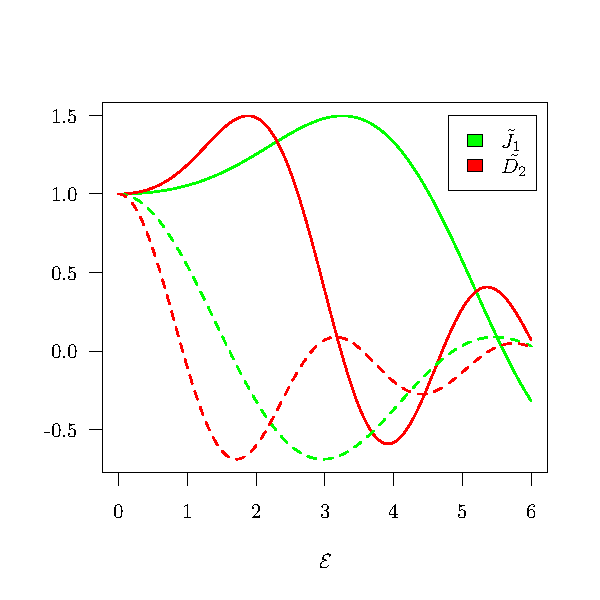
\includegraphics[width=\textwidth]{../Figures/NNvsNNN1.pdf}
  \end{minipage}\hfill
  \begin{minipage}[c]{0.5\textwidth}
    \caption{$\frac{J_{1}}{J_{1}^0}$ and $\frac{D_{2,ij}}{D_{2,ij}^0}$ are plotted as function of $\mathcal{E}$. Similar results are obtained in \cite{Mentink2015} for $J_{1}$. Solid lines are for $\omega = 4$ and dashed lines are for $\omega = 14$.}
  \end{minipage}
\end{figure}
\footfullcite{Mentink2015}
\end{frame}

%------------------------------------------------

\begin{frame}
\Huge{\centerline{The End}}
\end{frame}

\end{document}